%%
%%                  TEMPLATE for Math 436 project report
%%
\documentclass[11pt]{amsart}
%%% WARNING: Do NOT change the page size, fonts, or margins!  Penalties will apply.


\usepackage{graphicx}
\usepackage{amssymb,amsmath,amsthm}
\usepackage{placeins} %enables \FloatBarrier, which prevents figures and tables from going below it.
\usepackage{hyperref} %makes cross references into hyperlinks. 
\usepackage[utf8]{inputenc}
\usepackage{textcomp}
\usepackage{newunicodechar}

 

%%% WARNING: Do NOT change the page size, fonts, or margins!  Penalties will apply.
%%% WARNING: Do NOT change the page size, fonts, or margins!  Penalties will apply.

\begin{document}

\title{Modeling the Effects of Human Policy on Wolf--Elk Population Dynamics}
\author{Adam Eubanks, Ryan Haines, Norman Rasmussen, Jed Woods}

% Change the date to match the date you actually wrote this paper
\date{18 November 2026} % or use \today

\maketitle % this actually makes the title

\begin{abstract}
How does public policy impact an environment's predator-prey populations? In this paper, we apply Lotka-Volterra modeling concepts to elk and wolf populations under various Federal policies regarding farming, hunting, and the protection of these animals. We investigate how humans, as hunters, farmers, and trappers, influence the equilibrium of these ecosystems. Specifically, we investigate and model the wolf's extinction and subsequent return to Yellowstone. To enhance our predator-prey dynamics, we also add Beddington-DeAngelis to our modeling. We conclude that policy surrounding hunting and agriculture has huge cascading effects on the wolf-elk ecosystem that can be viewed almost immediately.
\end{abstract}

%% First Section
\section{Background/Motivation}


The reintroduction of wolves to Yellowstone National Park represents one of the greatest success stories of ecological policy. Federal policy against wolves resulted in their extinction from the Yellowstone area for a period of 70 years \cite{nps_wolf_history}. During this time, the elk population surged to nearly 20,000 animals \cite{nps_elk}. This resulted in severe over-grazing that destabilized the ecology of the whole park \cite{nps_cycles,ripple2012}. In response, Federal agencies reintroduced the native apex predator to Yellowstone, resulting in a ``trophic cascade'' that promulgated throughout the whole food chain \cite{nps_wolf_history,ripple2012}. With a present population of 70-80 wolves, Yellowstone's elk population has stabilized to $\sim$5,500 animals \cite{nps_wolf_management,nps_elk,nps_wolf_elk_2024}. By increasing vegetation through predation, the reintroduction of wolves has even improved seemingly non-related parts of the ecosystem, such as the beaver population, various bird populations, and flooding \cite{ripple2012,nps_beaver,baril2011}.

Contrasting Yellowstone's fierce protections of their wolf population, the State of Utah takes a very different approach \cite{nps_wolf_management,utah_wolf_plan}. Under Utah's Wolf Management Plan, wolves that encroach upon livestock are often subject to lethal removal \cite{utah_wolf_plan,utah_wolves}. In addition, the state manages its elk population through the distribution of game tags in the winter \cite{utah_drawings}. Thus, Yellowstone and the State of Utah both take very different approaches to managing their ecologies, with Yellowstone focused on conservation and Utah focused on conservation within the bounds of human agriculture and gaming \cite{nps_wolf_management,utah_wolf_plan,utah_drawings}.

We attempt to model these dynamics between wolves, elk, farmers, hunters, and available vegetation to motivate policy for an anthropocentric ecosystem.

Additionally, we include a Beddington--DeAngelis functional response to our Lotka--Volterra predator-prey system \cite{beddington1975,deangelis1975}, incorporating interference among predators (hunters and wolves going after the same elk) as well as prey density (hunting is easier when prey are closer together) \cite{beddington1975,deangelis1975}. We also include how farmers change carrying capacity by siphoning off land for livestock and crops:

\begin{align*}
\frac{dE}{dt} &= rE\left(1-\frac{E}{K_F}\right)
-\frac{aEW}{1+ahE+cW}-h_EE \\
\frac{dW}{dt} &= \frac{baEW}{1+ahE+cW}
-mW-h_WW-p_FW
\end{align*}

In this framework, new control variables reflect human policy choices:

\begin{itemize}
    \item \textbf{$K_F$}: The social or agricultural carrying capacity of the elk population. This value is modulated by farmer land-use; as farmers take up vegetation for domestic livestock or crops, $K_F$ decreases relative to the maximum environmental capacity.

    \item \textbf{$h_E$}: The per capita hunting rate of elk by human hunters.

    \item \textbf{$h_W$}: The per capita hunting rate of wolves by human hunters.

    \item \textbf{$p_F$}: The lethal removal rate of wolves driven by livestock protection policies \cite{utah_wolves,utah_wolf_plan}.
\end{itemize}


% \begin{figure}[htb]
% \begin{center} %Put your images in a figure like this
% \includegraphics[width=\textwidth]{Myfig.pdf} % Better to make them pdfs than png or gif or jpeg
% \end{center}
% \caption{Plots should be high resolution (pdf 300dpi), uncluttered, a reasonable size, and easily readable and understandable. If you make plots in MatPlotLib, be sure to set the \texttt{figsize} option to be the actual size in inches that your final figure will be in the LaTeX document (so width 5 for a full-width figure).  Otherwise when you put your figure in your document it will scale the text to be a bad size---either too big or too small.  All figures should have a complete caption that helps the reader make sense of the figure even if they haven't read the paper yet. Here is an example: This figure shows the risk or mean squared error (in black) of for a generic family of regression models as a function of model complexity (the number of free parameters in the model).  The generalized aliasing decomposition shows that the risk is the sum of three parts: Model insufficiency (red), Data insufficiency (green), and Aliasing (blue).  Model insufficiency is monotonically decreasing as a function of complexity, Data insufficiency vanishes when the number of parameters is less than the number of training points (the classical regime), but increases monotonically in the modern regime (where the number of parameters is greater than the number of data points).  Aliasing generally increases up to the interpolation threshold and decreases thereafter, converging to zero almost surely as the number of parameters goes to infinity.  
% }
% \label{fig:MeanSquaredError} % for automatic cross referencing
% \end{figure}



%% Second Section 
\section{Modeling}

We choose to begin with a basic model.
This ODE models elk population ($E$) and wolf population ($W$).
We included many elements and assumptions from the classic predator-prey model such as: a carrying capacity for the elk, elk hunted by wolves, wolf birth rate determined by number of elk, and a wolf death rate. Beyond this, we add three additions to our baseline model. First, we assume that the farmers will make use of available land and therefore decrease the carrying capacity of the elk, which we represent by $K-\alpha_{FE}F$. We also assume that farmers will kill wolves to stop them from killing livestock, so we add $c_{FW}FW$. Finally, we assume that hunters will hunt elk and add $c_{HE}HE$. This all comes together to form our basic model:
\begin{equation}
\begin{aligned}
\frac{dE}{dt}
&= r_E E\left(1-\frac{E}{K-\alpha_{FE}F}\right)
-aEW-c_{HE}HE,\\
\frac{dW}{dt}
&= \eta aEW-d_WW-c_{FW}FW.
\end{aligned}
\end{equation}

\begin{itemize}
    \item $E(t)\geq0$: Elk population at time $t$.
    \item $r_E >0$: Growth rate of elk.
    \item $K>0$: Natural carrying capacity of the elk population.
    \item $W(t)\geq0$: Wolf population at time $t$.
    \item $a>0$: Wolf predation rate coefficient on elk.
    \item $\eta>0$: Conversion efficiency of consumed elk into wolf population growth.
    \item $d_W>0$: Mortality rate of wolves.
    \item $F\geq0$: Constant farmer pressure.
    \item $\alpha_{FE}\geq0$: Reduction in elk carrying capacity per unit of farmer pressure.
    \item $c_{FW}\geq0$: Wolf mortality rate per unit of farmer pressure.
    \item $H\geq0$: Constant hunter pressure.
    \item $c_{HE}\geq0$: Elk mortality rate per unit of hunter pressure.
\end{itemize}

Performing simple algebra we can find the equilibrium points

\begin{enumerate}
    \item \textbf{Extinction equilibrium:}
    \[
    (E,W) = (0,0).
    \]

    \item \textbf{Elk-only equilibrium:}
    \[
    (E,W) = \left(\frac{Cm}{r_E},0\right).
    \]

    \item \textbf{Coexistence equilibrium:}
    \[
    (E,W) =
    \left(
    \frac{q}{\eta a},
    \frac{m}{a}-\frac{r_E q}{\eta a^2 C}
    \right).
    \]
\end{enumerate}

where
\[
C = K-\alpha_{FE}F,\qquad
m = r_E-c_{HE}H,\qquad
q = d_W+c_{FW}F.
\]
The Extinction equilibrium represents when both populations become 0 and go extinct. The Elk-only equilibrium represents the case when the wolves go extinct leading the elk to reach their carrying capacity. Finally, the Coexistence equilibrium is the case when both populations exist together. Using linearization techniques we get the cases for when each equilibrium point exists on the positive plane (negative populations do not exist), are asymptotically stable, and stable. We provide a graph in Figure \ref{fig:fig1} illustrating the flow of this ODE.


\begin{table}[h]
\centering
\small
\renewcommand{\arraystretch}{1.8}
\begin{tabular}{|c|c|c|c|}
\hline
\textbf{Equilibrium} &
\textbf{Nonnegative Plane} &
\textbf{Asymptotically Stable} &
\textbf{Stable Only} \\
\hline

$(0,0)$ &
Always &
$m \leq 0,\ q>0$ &
$m \leq 0,\ q=0$ \\
\hline

$\left(\frac{Cm}{r_E},0\right)$ &
$m>0$ &
$q \geq \frac{\eta a Cm}{r_E}$ &
Never \\
\hline

$\left(
    \frac{q}{\eta a},
    \frac{m}{a}-\frac{r_E q}{\eta a^2 C}
    \right)$ &
$q>0,\ \eta aCm>r_Eq$ &
$q>0,\ \eta aCm>r_Eq$ &
Never \\
\hline
\end{tabular}
\caption{Existence and local stability of equilibrium points.}
\end{table}

\begin{figure}
    \centering
    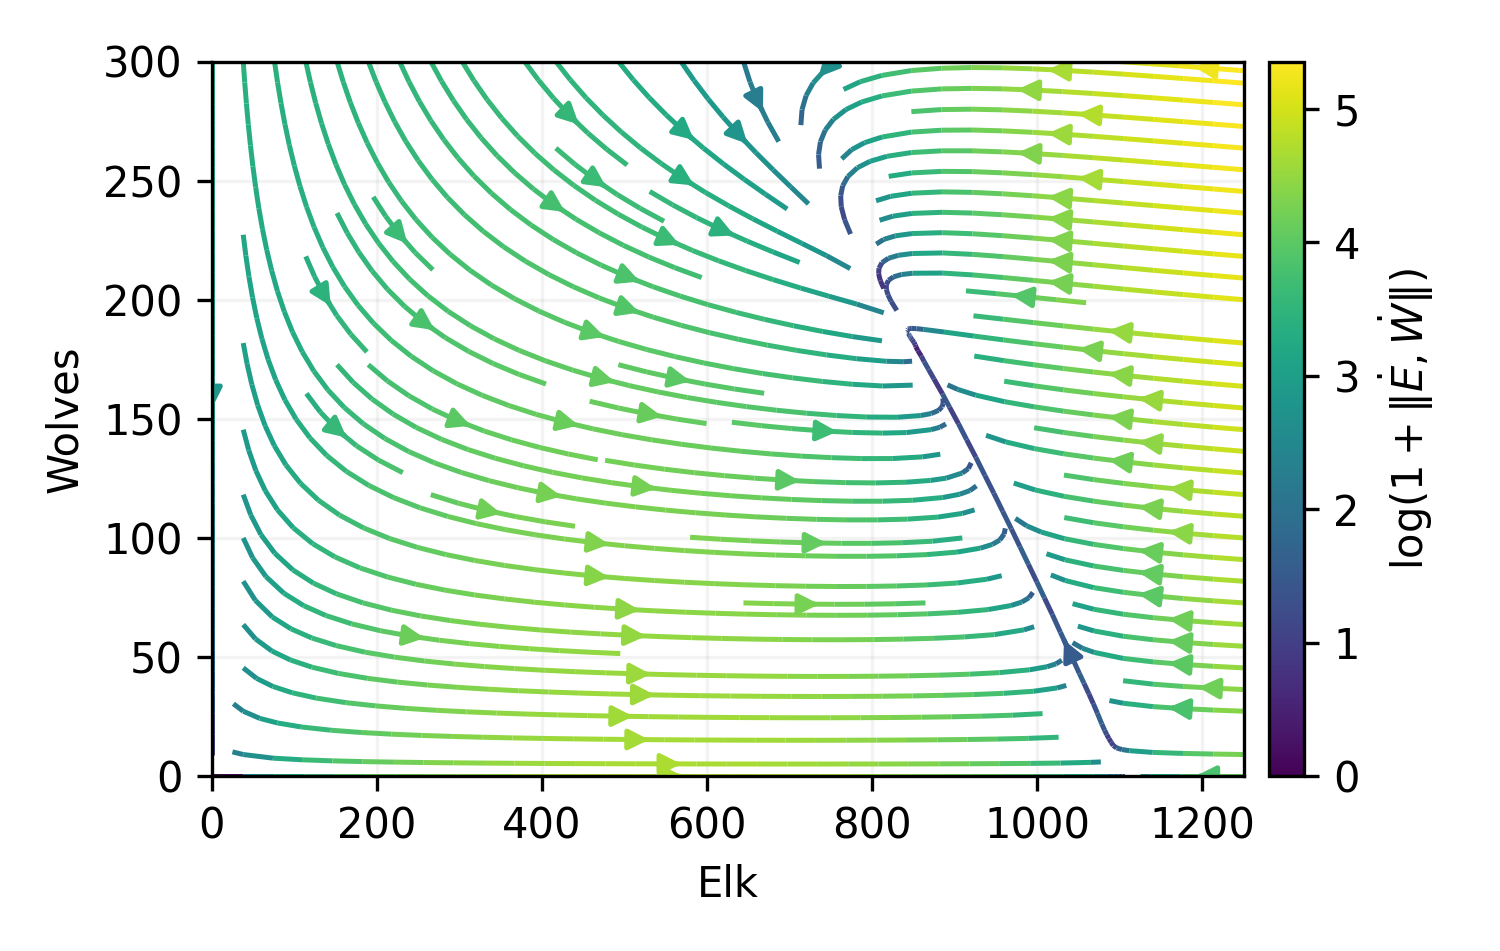
\includegraphics[width=1\linewidth]{simple_model_flow.png}
    \caption{Phase-plane flow of the simple wolf-elk model. Streamlines show the direction of population change, and color indicates $\log(1+\text{speed})$. Parameters are $r_E=0.40$, $K=1200$, $\alpha_{FE}=10$, $a=0.001$, $\eta=0.25$, $d_W=0.08$, $F=6$, $H=4$, $c_{HE}=0.003$, and $c_{FW}=0.004$.}
    \label{fig:fig1}
\end{figure}




\subsection{Frontier Expansion}

One of the first ideas we had was to try to model a "frontier expansion", imagining farmers and hunters settling a new area. To model this, we assumed that the expansion would start at 0\% and end with 100\%. We added a function $u(x):\mathbb R \to [0,1]$  to show how this expansion occurs. We used 3 variations:
\[
u(t)=\operatorname{clip}\!\left(\frac{t-t_0}{D},\,0,\,1\right),
\qquad D>0,
\]
\[
\begin{aligned}
f_{\mathrm{linear}}(u) & = u,\\[4pt]
f_{\mathrm{exponential}}(u) & = \frac{e^{4u}-1}{e^4-1},\\[4pt]
f_{\mathrm{arctangent}}(u) & =
\frac{\arctan\!\bigl(4(2u-1)\bigr)+\arctan(4)}
     {2\arctan(4)}.
\end{aligned}
\]
The linear function represents a baseline, the exponential a slow start that picks up momentum, and the arctangent a slow pickup then slowdown at the end. A graph of these functions is provided in Figure \ref{fig:fig2}.

\begin{figure}
    \centering
    \includegraphics[width=1\linewidth]{frontier_introduction_schedules.png}
    \caption{Linear, exponential, and arctangent schedules for introducing farmer and hunter pressure. Each curve shows the fraction of maximum pressure over time: introduction begins at $t=10$ and reaches full pressure at $t=45$. Dashed lines mark these times.}
    \label{fig:fig2}
\end{figure}

We hoped that we would see that adding this slow introduction would change the behavior of the model, perhaps showing that a slow introduction would preserve an ecosystem while fast introduction would destroy it. However, this was not the case as seen in Figures \ref{fig:fig3} and \ref{fig:fig4}. Figure \ref{fig:fig3} shows how the introduction parameters do not change the equilibrium, and Figure \ref{fig:fig4} shows how the introduction causes convergence to the equilibrium to take much more time. 

\begin{figure}
    \centering
    \includegraphics[width=1\linewidth]{frontier_introduction_population_response.png}
    \caption{Elk and wolf population responses to linear, exponential, and arctangent introductions of farmer and hunter pressure. As you can see each introduction method has slightly different curves, but settles on the same equilibrium. Each simulation starts at $(E,W)=(600,50)$; pressure rises from zero at $t=10$ to its maximum at $t=45$, with $F_{\max}=40$ and $H_{\max}=25$. This figure uses the same parameters as Figure~\ref{fig:fig2} except for $F_{\max}$ and $H_{\max}$.}
    \label{fig:fig3}
\end{figure}

\begin{figure}
    \centering
    \includegraphics[width=1\linewidth]{playground2_wolf_vs_elk.png}
    \caption{Wolf--elk phase-plane trajectories comparing gradual pressure introduction with full farmer and hunter pressure from the start. It is clear that the non-introduction case converges to the equilibrium much faster than the gradual introduction case. 
    Both simulations begin at $(E,W)=(650,110)$. In the gradual case, pressure follows a smoothstep ramp from $t=10$ to $t=11$; in the full-force case, $F=40$ and $H=25$. This figure uses the same parameters as Figure~\ref{fig:fig2} except for $F_{\max}$ and $H_{\max}$.}
    \label{fig:fig4}
\end{figure}


\subsection{Wolf Reintroduction}

Keeping the constants the same from the previous wolf extinction model, we next explore the policy that wolves were able to be reintroduced into Yellowstone. According to the National Park Service, they took wolves from around the area and reintroduced them in groups of about 15 at a time. To model this, we added a release rate variable $R(t)$ that did not depend on $W$. At time steps we chose, we added 15 wolves at a time and wanted to see how this would affect our model. Also, with the reintroduction of wolves, they added a policy where the wolves could not be killed and were protected on Yellowstone land. We accounted for this with a factor $\phi(t)$ that can be turned on or off. We turn off the protection by adding a zero to the farmer killing rate and the wolf hunter rate. With these removed, we see that the wolves do not have a problem bringing the elk population down to a new equilibrium where both wolves and elk are stable.
\begin{equation}
    \frac{dW}{dt}
=
\frac{baEW}{1 + ahE + cW}
- mW
- \phi(t)(h_W + p_F)W
+ R(t).
\end{equation}


\begin{figure}
    \centering
    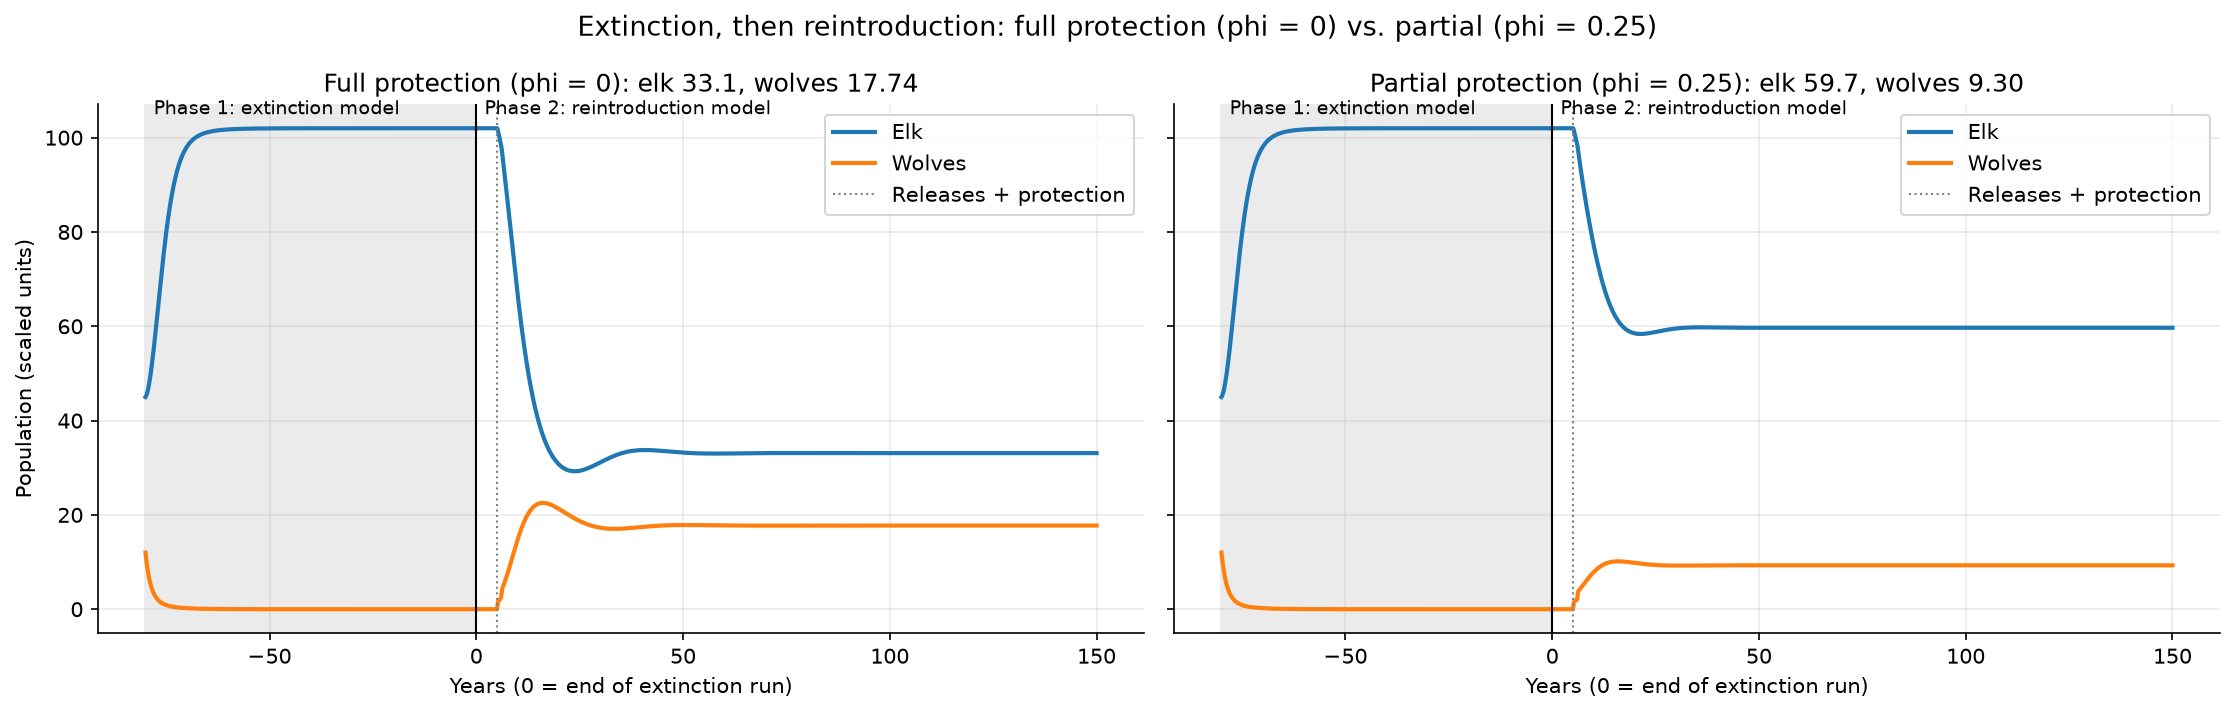
\includegraphics[width=1\linewidth]{reintroduction_phi_0_vs_025_populations.png}
    \caption{Wolf and elk populations through extinction and reintroduction
under full protection (left, $\phi = 0$) and partial protection
(right, $\phi = 0.25$). Phase 1 (shaded): heavy human-caused wolf
mortality drives wolves functionally extinct, and elk grow to their
wolf-free level of approximately $102$. Phase 2: approximately
$30$ wolves are released in years $5$ and $6$, and protection begins.
Under full protection, wolves overshoot to approximately $225$ and
settle at $177$ ($17.7$ units), while elk fall to $33$.
Under partial protection, wolves settle at approximately $93$
($9.3$ units) and elk at $60$. Protection strength determines how
many wolves the system supports, not how quickly they recover.
Populations are expressed in scaled model units
($1$ wolf unit $\approx 10$ wolves).}
    \label{fig:fig5}
\end{figure}


We see that, with simple reintroduction and various numbers of wolves that we release, the wolves and elk will ultimately reach this new protected equilibrium shown below 


\begin{figure}
    \centering
    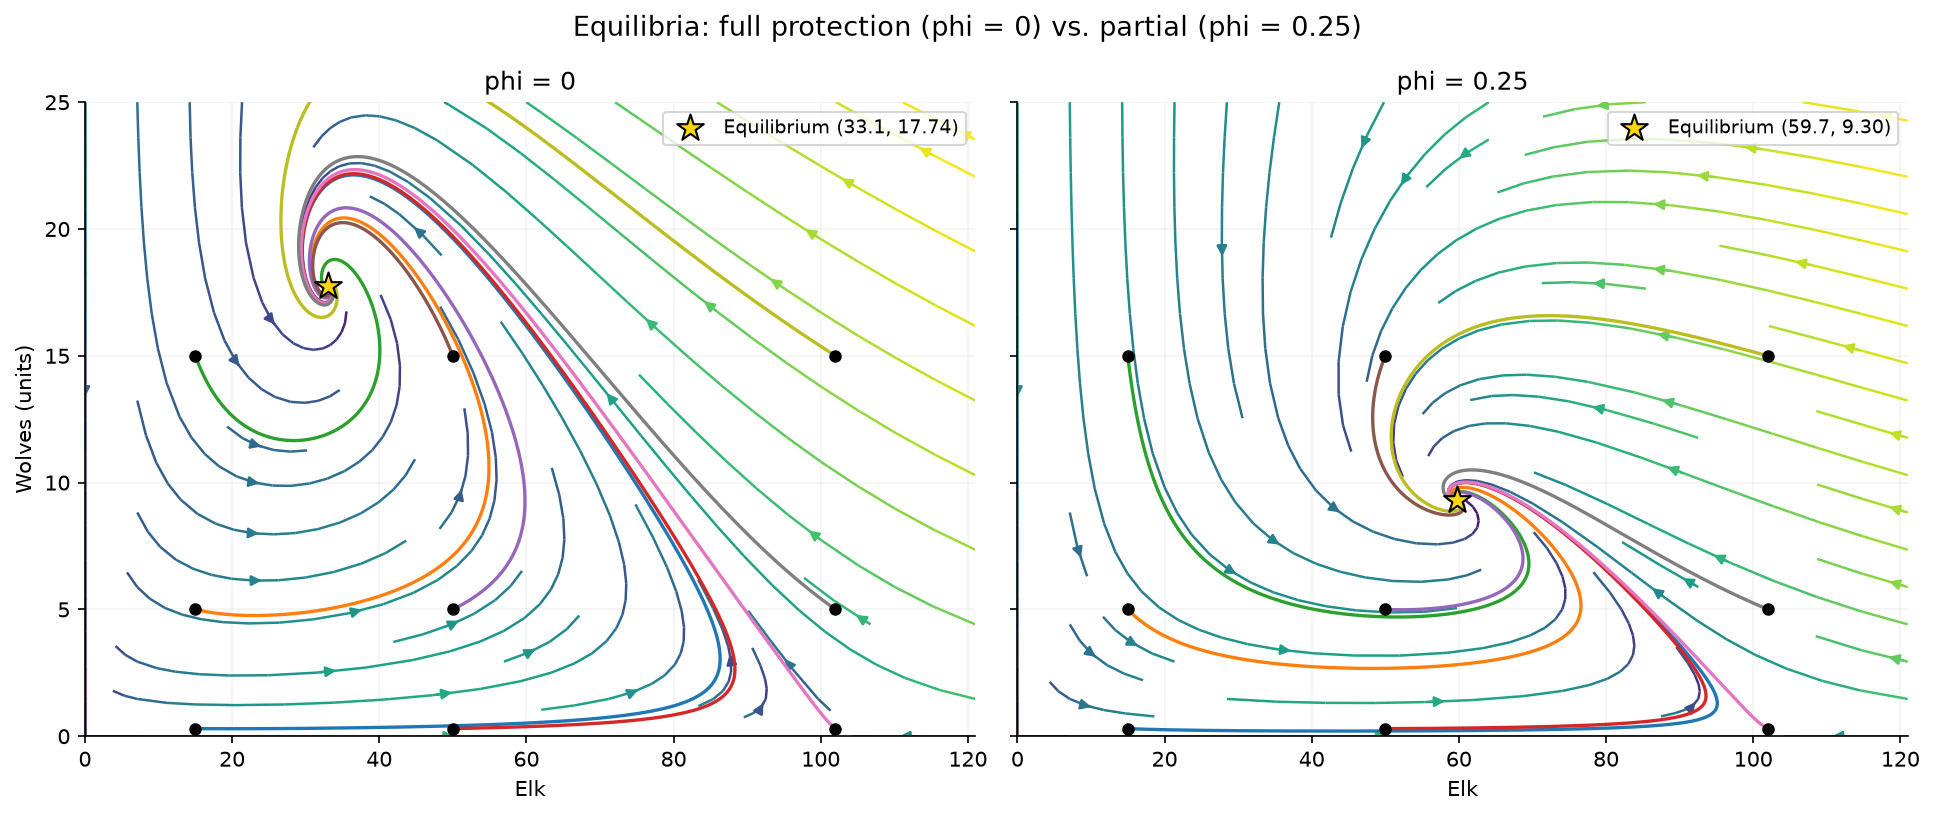
\includegraphics[width=1\linewidth]{reintroduction_phi_0_vs_025_equilibria.png}
    \caption{Phase planes of the wolf--elk model under full protection
(left, $\phi = 0$) and partial protection (right, $\phi = 0.25$),
with no further releases. Streamlines indicate the direction of
the flow. Colored curves represent trajectories from nine initial
conditions (black dots), combining low, medium, and high elk
populations ($15$, $50$, $102$) with low, medium, and high wolf
populations ($0.3$, $5$, $15$ units). In each case, every trajectory
spirals toward a single stable coexistence equilibrium (star).
Under full protection, the equilibrium is approximately
$(E^*, W^*) = (33, 17.7)$, corresponding to $33$ elk and
approximately $177$ wolves. Under partial protection, the
equilibrium shifts to approximately $(E^*, W^*) = (60, 9.3)$,
corresponding to $60$ elk and approximately $93$ wolves.
Weaker protection shifts the equilibrium toward more elk
and fewer wolves, but all trajectories converge to the same
equilibrium within each protection scenario.}
    \label{fig:fig6}
\end{figure}



\subsection{Wolf Hunting Policies}

The underlying dynamics are a predator--prey system for elk and wolves. Elk grow subject to a carrying capacity, wolves recruit through predation on elk, and both populations experience natural mortality. In the trapping experiments, farmers are set to zero so that the only additional human pressure on wolves is hunting. This isolates the effect of harvest rules on the coupled populations.
Hunting effort is updated periodically rather than continuously. At the start of each decision interval, effort is computed from the wolf abundance recorded at the previous decision and is then held fixed until the next update. Wolf losses due to hunting increase with both current wolf abundance and current effort.
\subsubsection{Tracked adaptive policy}
The managed (tracked) rule is abundance-dependent. When the lagged wolf census exceeds a prescribed target, effort is increased; when abundance falls below the target, effort is reduced, subject to a lower bound of zero and an upper cap. Under the default parameters, this feedback produces a stable positive wolf population and a correspondingly stable elk trajectory. In that regime, the policy functions as a control mechanism that regulates wolf density rather than driving the predator to extinction.
\subsubsection{Untracked harvest}
A second scenario retains the same tracked rule and adds an independent, stochastic component of wolf removal. This term represents harvest outside the managed quota, such as unreported take. Importantly, the noise enters through removals, not through observation error in the census: managers still respond to the true lagged count, but total hunting pressure is the sum of managed effort and untracked effort.
Because untracked removals can remain positive even when the managed policy has already reduced legal effort, the stabilizing feedback of the tracked rule can be weakened or overridden.
\subsubsection{Role of the policy in the system}
The policy matters because it introduces a state-dependent human feedback into the ecological model. Equilibrium behavior and stability therefore depend not only on biological parameters, but also on policy parameters such as the abundance target, the responsiveness of effort to deviations from that target, the length of the decision interval, and effort caps.
Under the tracked policy alone, the defaults support coexistence. When the same policy is supplemented by untracked harvest, outcomes become path-dependent: in some realizations wolves persist at reduced abundance, while in others they fall below a quasi-extinction threshold and remain extinct. After wolf extinction, elk increase toward carrying capacity, consistent with release from predation. The principal long-run ecological consequence is therefore loss of the predator population, not collapse of elk.
These comparisons indicate that an apparently adequate managed harvest rule can fail once removals include a component outside managerial control. Evaluating hunting policy in this system therefore requires accounting for both the formal control rule and additional untracked pressure on wolves.
\begin{figure}
    \centering
    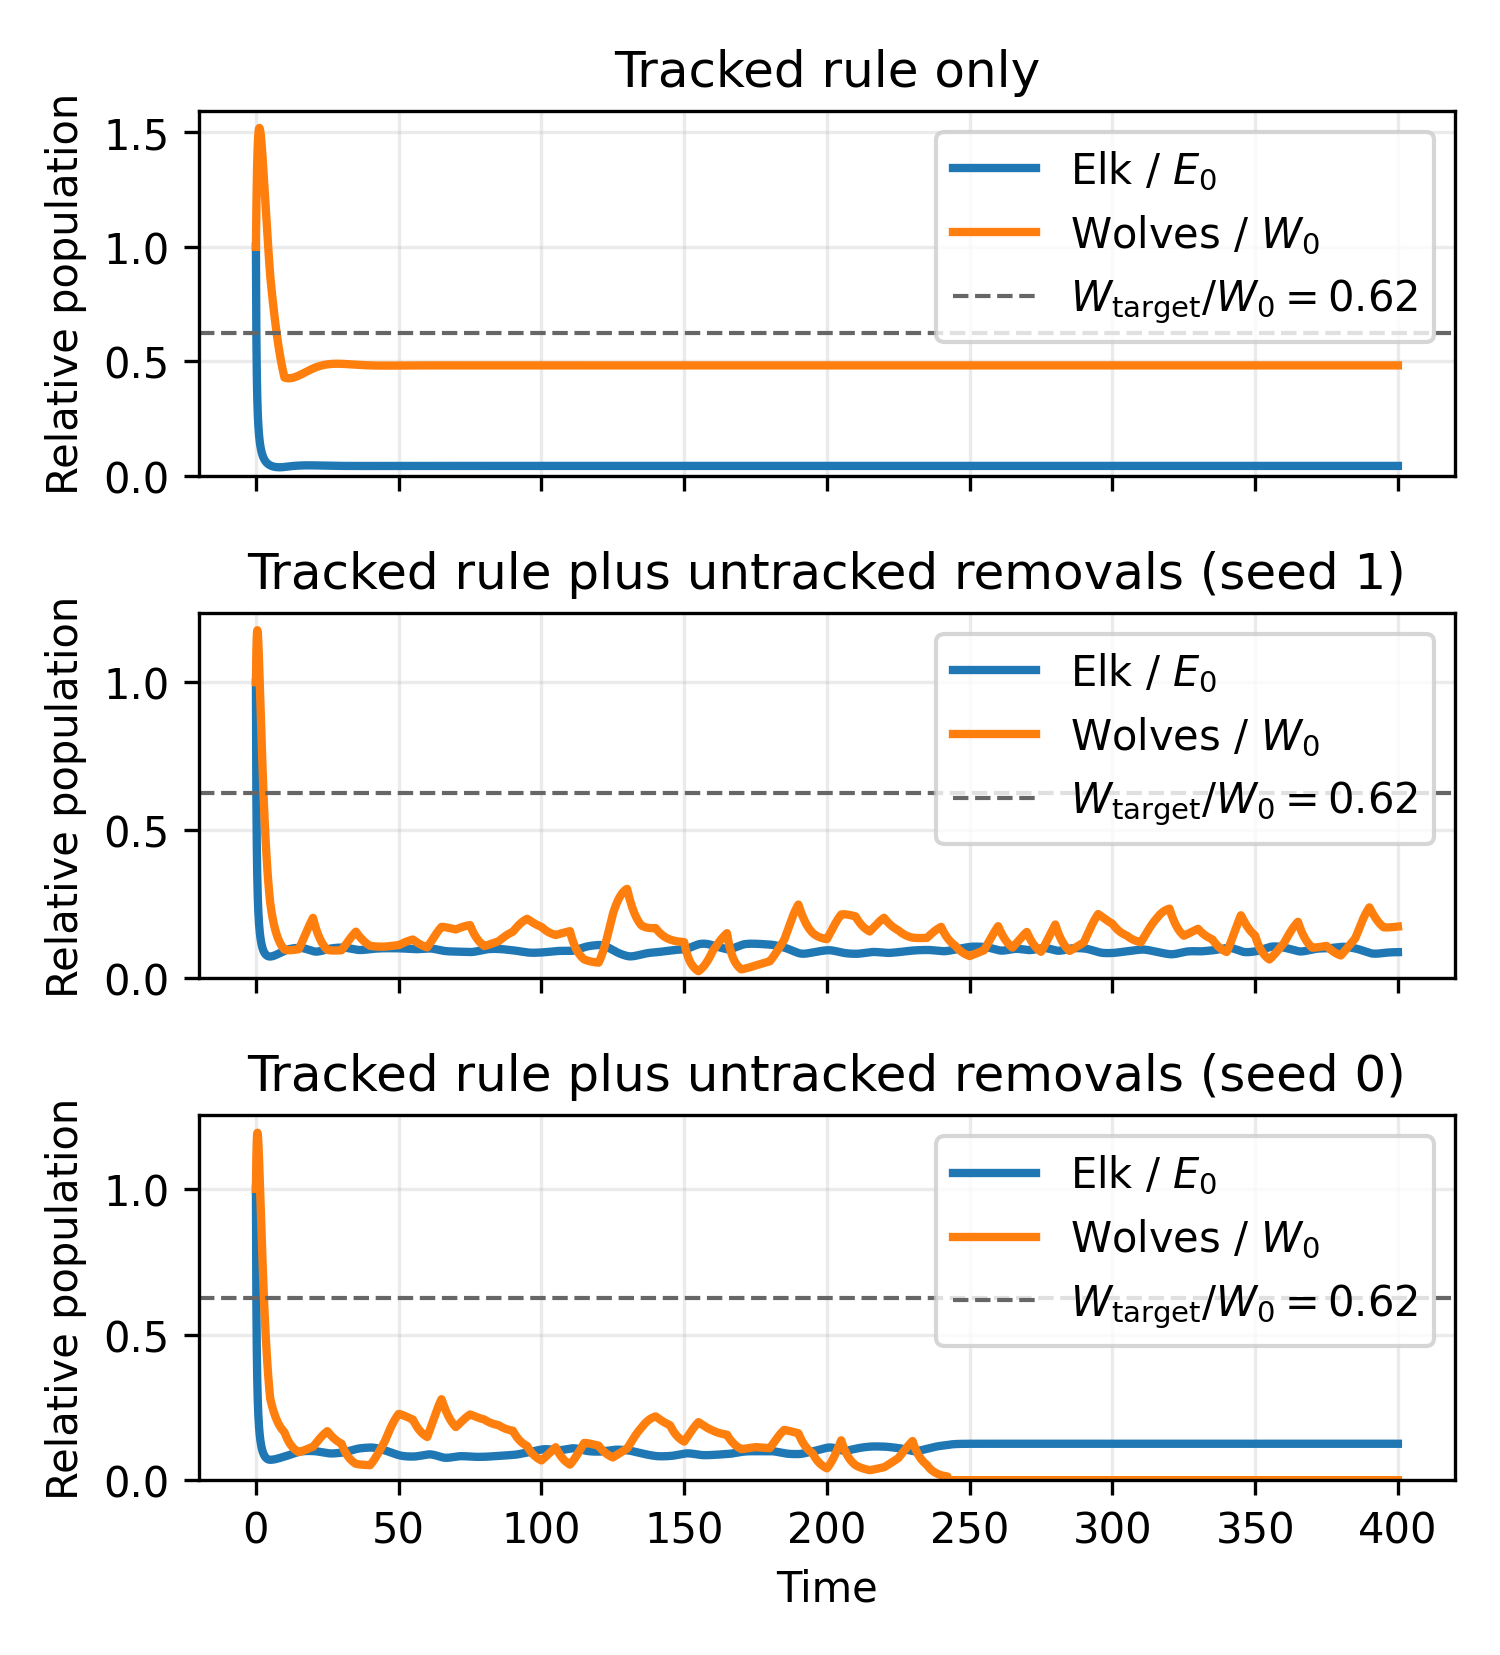
\includegraphics[width=1\linewidth]{trapper_policies_comparison.png}
    \caption{Elk and wolf counts are shown relative to their starting values under a hunting rule that raises effort when the lagged wolf census is above a target and lowers it when the census is below. The top panel uses only that tracked rule and both populations stay positive, while the middle and bottom panels add random untracked wolf removals and show one case where wolves persist and one where they go extinct.}
    \label{fig:fig7}
\end{figure}




%% Third Section
\section{Results}

% Clearly and succinctly state and describe the conclusions that you can draw from the model you have achieved (or the many failed attempts), and your numerical simulations.  Does your model(s) perform well quantitatively or qualitatively?

%%Fourth Section
\section{Analysis/Conclusions}

Wolf Extinction Analysis:
When wolves go extinct, the elk population quickly shoots up to the carrying capacity. However, the carrying capacity is susceptible to overgrazing, as shown in Figure~\ref{fig:fig8}.
\begin{figure}
    \centering
    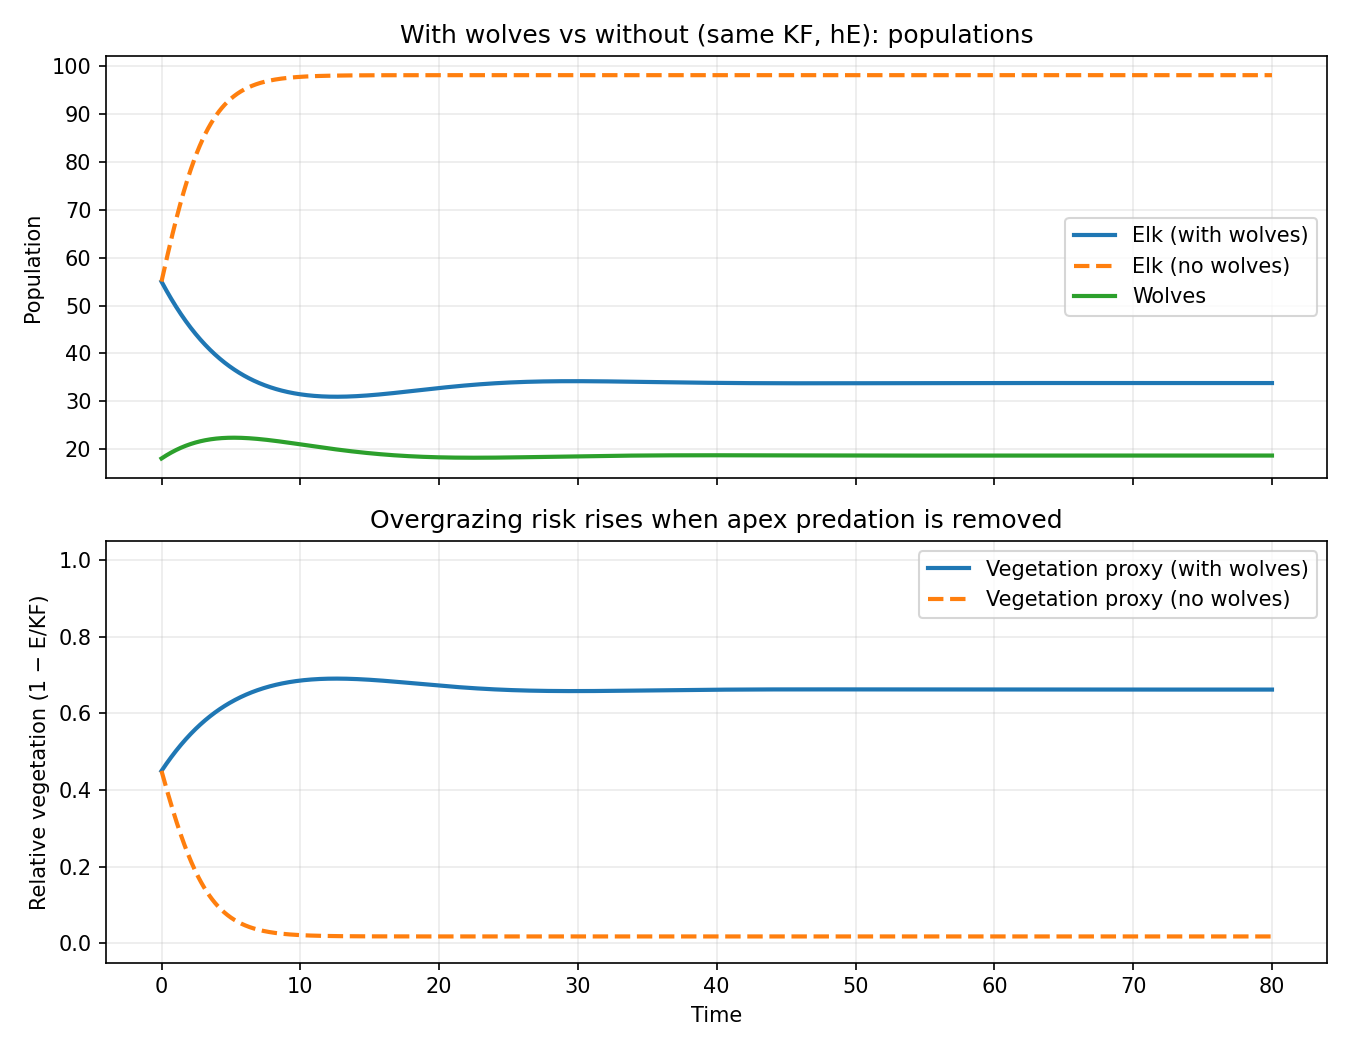
\includegraphics[width=1\linewidth]{wolf_extinction_comparison.png}
    \refstepcounter{figure}\label{fig:fig8}
\end{figure}

The presence of wolves greatly decreases the elk population below carrying capacity, preventing overgrazing. We find that farmer-induced extinction of wolves similarly rapidly increases elk population to carrying capacity. Even when farmers slowly get rid of wolves, as shown in Figure~\ref{fig:fig9}, the elk still shoot up to a level that would likely produce overgrazing.

\begin{figure}
    \centering
    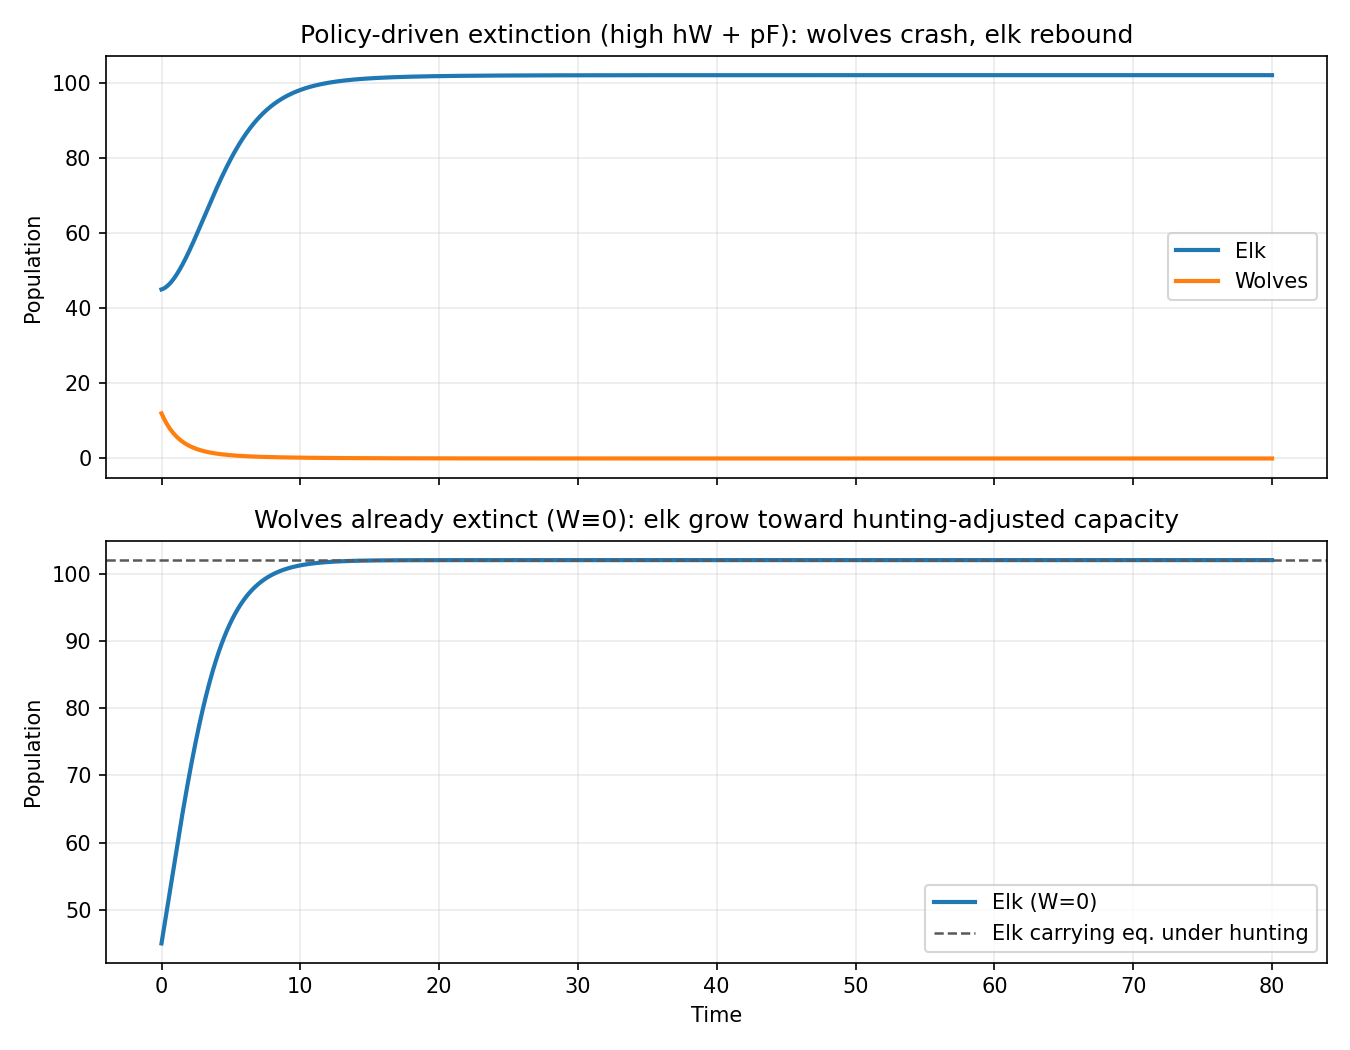
\includegraphics[width=1\linewidth]{wolf_extinction_timeseries.png}
    \refstepcounter{figure}\label{fig:fig9}
\end{figure}


\section{AI Disclosure}

We used AI to help accelerate code production, experimentation, and translating our models to LaTeX. It also helped find resources for our literature review and explore the space adjacent to our research. This helped to iterate faster, validate models and plot the results among other things.  The ideas presented, modeling decisions, theoretical explorations and conclusions were ours. 

\vspace*{1in}
This part should all be done before you get to \emph{page 11}.  The bibliography can spill on to page 11, but we won't read text or look at figures that go past the end of page 10.


%%%%%%%%%%%%%%%%%%%%%%%%%%%%%%%%%%%%%
%% Bibliography below
%%%%%%%%%%%%%%%%%%%%%%%%%%%%%%%%%%%%%
\FloatBarrier % Keep the figures from being put after the bibliography
\newpage
%% If using bibtex, leave this uncommented
\bibliography{refs} %if using bibtex, call your bibtex file refs.bib
\bibliographystyle{alpha}

%% If not using bibtex, comment out the previous two lines and uncomment those below
%\begin{thebibliography}{99}
%\bibitem{Vandermeersch} First reference goes here
%\end{thebibliography}

\end{document}
